\documentclass{article}
\usepackage{float}
\usepackage{hyperref}
\usepackage[utf8]{inputenc}
\usepackage{graphicx}
\usepackage{caption}
\usepackage{subcaption}
\usepackage{algpseudocode}
\usepackage{algorithm}
\usepackage{mathtools}
\usepackage{amsmath,amssymb}
\usepackage{siunitx}
\usepackage{listings}
\usepackage{bbm}
\usepackage[most]{tcolorbox}
\newcommand{\e}[1]{{\mathbb E}\left[ #1 \right]}
\definecolor{block-gray}{gray}{0.90}
\newtcolorbox{code}{colback=block-gray,grow to right by=-1mm,grow to left by=-1mm,boxrule=0pt,boxsep=0pt,breakable}
\lstset{
  basicstyle=\ttfamily,
  columns=fullflexible,
  frame=single,
  breaklines=true,
  postbreak=\mbox{\textcolor{red}{$\hookrightarrow$}\space},
}

\title{\vspace{-3cm}Charlie meeting 16th May\vspace{-3em}}
\author{}
\date{}

\begin{document}
\maketitle
\section*{Discussed and Processed}
As a running example, we consider a 1D simple harmonic oscialltor with force $kq$, where $q$ is the position.
Now we have observation as a series of data $\mathcal{D}$ from the observation of trajectories, $\mathbf{x_t}$, where 
\begin{equation*}
 \mathbf{x_t} = 
 \begin{pmatrix}
  q_t \\
  \dot{q}_t \\
\end{pmatrix} 
\end{equation*}
with $q_t$ being positional data and $\dot{q}_t$ being th velocity at time $t$. 
We can describe the system dynamics with this equation $\mathbf{\dot{x_t}} = v(\mathbf{x_t})$.
In our case, 
\begin{equation*}
  v=
  \begin{bmatrix}
    0 & 1 \\
    -\frac{k}{m} & 0\\
  \end{bmatrix}
\end{equation*}
so that 
\begin{equation*}
  \begin{bmatrix}
    \dot{q_t} \\
    \ddot{q}_t\\
  \end{bmatrix}
  =
  \begin{bmatrix}
    0 & 1 \\
    -\frac{k}{m} & 0\\
  \end{bmatrix}
\begin{bmatrix}
  q_t \\
  \dot{q_t}
\end{bmatrix}
\end{equation*}

If we are able to get the dynamics $v$, we will then be able to predict the trajectories.
\newline
However, if we only have position data $x_t$ and not the velocity, we instead write $\dot{x}_t = \frac{d x_t}{d t} = v(x_t)$, which if we have $v$, we can again use it to update the $x_t$. 
In our case, $v(x)=\pm\sqrt{\frac{2H}{m}-\frac{kx^2}{m}}$, where $H$ is the Hamiltonian or Energy term. 

Now, if we define an arbitrary function $F$ as a function of the d-dimensions space $x_t$ only and does not depend on time $t$ explicitly and only depends on $v=\dot{x}$ through $x$, $v(x_t)$, $F(x_t)$, we have that by chain rule 
$$\frac{dF(x_t)}{dt} = \frac{dx_t}{dt} \nabla_x (F(x_t)) = v(x_t)\cdot\nabla_x(F(x_t)),$$
If we wish for F to be an invariance (e.g. energy, momentum), we then proceed to write $\mathcal{L} = v\cdot\nabla$ such that $\mathcal{L}[F]=0$.
As a result, the invariance will lie in the null space of $\mathcal{L}$.
Since to get the real form of $\mathcal{L}$, we will be required to know the form of $v$, the dynamics, which we don't have; therefore, instead, we will need to approximate $\hat{\mathcal{L}}_{\Delta t}[F] \approx \frac{F(x_{t+\Delta t})-F(x_t)}{\Delta t}$ (since it is the time derivative).
We then put a GP prior on $F$ such that $F\sim\mathcal{GP}(0, K)$, where K is an appropriate covariance matrix.
Since the $\hat{\mathcal{L}}_{\Delta t}$ is linear, $\hat{\mathcal{L}}_{\Delta t}[F]$ will also be a GP with form $\hat{\mathcal{L}}_{\Delta t}[F]\sim \mathcal{GP}(0, \hat{\mathcal{L}}_{\Delta t}^{\dagger}K\hat{\mathcal{L}}_{\Delta t})$ 
As a result, we can see the joint distribution of $F$ and $\hat{\mathcal{L}}_{\Delta t}[F]$ will be
\begin{equation*}
  \begin{pmatrix}
    F\\
    \hat{\mathcal{L}}_{\Delta t}[F]\\
  \end{pmatrix}
  \sim
  \mathcal{N}
  \left(
  \begin{pmatrix}
      0\\
      0\\
  \end{pmatrix}
  ,
  \begin{pmatrix}
    K & \hat{\mathcal{L}}_{\Delta t}K \\
    K\hat{\mathcal{L}}_{\Delta t}^\dagger & \hat{\mathcal{L}}_{\Delta t} K \hat{\mathcal{L}}_{\Delta t}^\dagger\\
  \end{pmatrix}
  \right)
\end{equation*}

Instead of conditioning on training data, we will then condition on $\hat{\mathcal{L}}[F]=0$, and the resulting F should be then the invaraince, up to an additive constant. 

We have the joint normal distribution condition formula.
$$
\begin{aligned}
p\left(\left[\begin{array}{l}
\mathbf{x}_{1} \\
\mathbf{x}_{2}
\end{array}\right]\right) &=\mathcal{N}\left(\left[\begin{array}{l}
\mathbf{x}_{1} \\
\mathbf{x}_{2}
\end{array}\right] ;\left[\begin{array}{l}
\boldsymbol{\mu}_{1} \\
\boldsymbol{\mu}_{2}
\end{array}\right],\left[\begin{array}{ll}
\boldsymbol{\Sigma}_{11} & \boldsymbol{\Sigma}_{12} \\
\boldsymbol{\Sigma}_{21} & \boldsymbol{\Sigma}_{22}
\end{array}\right]\right) \\
p\left(\mathbf{x}_{1} \mid \mathbf{x}_{2}\right) &=\mathcal{N}\left(\mathbf{x}_{1} ; \boldsymbol{\mu}_{1}+\boldsymbol{\Sigma}_{12} \Sigma_{22}^{-1}\left(\mathbf{x}_{2}-\boldsymbol{\mu}_{2}\right), \boldsymbol{\Sigma}_{11}-\boldsymbol{\Sigma}_{12} \boldsymbol{\Sigma}_{22}^{-1} \boldsymbol{\Sigma}_{21}\right)
\end{aligned}
$$
Therefore, we have 
$$
p(F|\hat{\mathcal{L}}_{\Delta t}[F]=0)\sim \mathcal{N}\left(0,K-\hat{\mathcal{L}}_{\Delta t}K(\hat{\mathcal{L}}_{\Delta t} K \hat{\mathcal{L}}^\dagger_{\Delta t} )^{-1}K\hat{\mathcal{L}}^\dagger_{\Delta t} \right)
$$

The resulting F should therefore be the invariant quantity up to an additive constant (which will disappear by time derivative)
After we get the invariances, we will need to constrain our dynamics such that it respects the invariance. 
For example, if energy is conserved, a harmonic oscialltor will be constrained on a circle in phase space.
We know that $v(x_t)\cdot\nabla_x F(x_t)=\nabla_x F(x_t) \cdot v(x_t) = 0$
If we use a simliar trick as discuessed earlier.
This time, again, we may not have the the exact form of $\nabla_x F(x_t)$ so we will replace that with the approximation $\hat{\nabla}_{\Delta x}F=\frac{F(x+\Delta x)-F(x)}{\Delta x}$(we can replace $\hat{\nabla}_{\Delta x}F$ with the exact form $\nabla_xF$ if available)
But this time we put a prior on $v(x_t)$ this time instead, and we condition on $\nabla_xF \cdot v=0$.
Therefore, if we place a GP prior on $v(x_t)\sim\mathcal{GP}(0, K)$, we will have $\nabla_xF \cdot v \sim \mathcal{GP}(0, \nabla^\dagger_xF K \nabla_xF)$ if $\nabla_xF$ is again linear (it may not always be linear with respect to $v$). 
We then have similarly, 
\begin{equation*}
  \begin{pmatrix}
    v\\
    \nabla_xF\cdot v\\
  \end{pmatrix}
  \sim
  \mathcal{N}
  \left(
  \begin{pmatrix}
      0\\
      0\\
  \end{pmatrix}
  ,
  \begin{pmatrix}
    K & \nabla_xF K \\
    K\nabla^\dagger_xF & \nabla_xF K \nabla_x^\dagger F\\
  \end{pmatrix}
  \right)
\end{equation*}

We will parametise $F$, and backpropagate such that the marginal likelihood is maximised. 
We know that $F$ is invariance in time.


Similar to before, we have 
$$
p(v|\nabla_xF\cdot v=0)\sim \mathcal{N}\left(0,K-\nabla_xFK(\nabla_xF K \nabla_x^\dagger F)^{-1}K\nabla_x^\dagger F\right).
$$


\begin{figure}[H]
  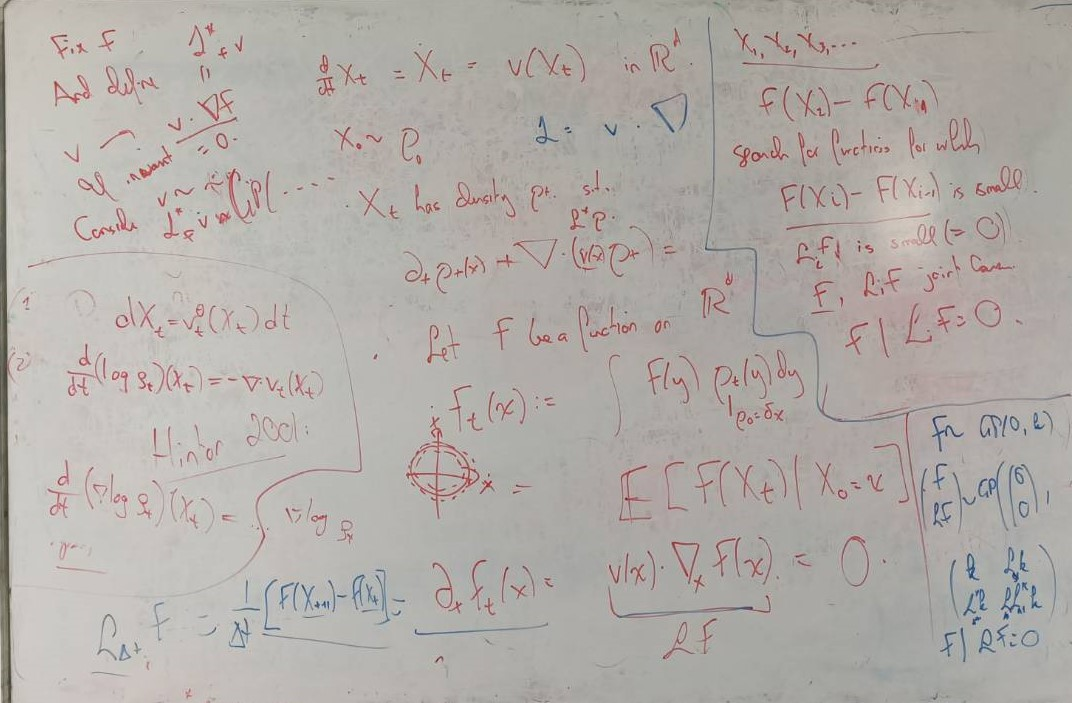
\includegraphics[width=\linewidth]{332800.jpg}
  \centering
\end{figure}

\section*{Next Step}
We will first test the inference performance assume given F, the invariance.
So say for 1D simple harmonic oscialltor, we have conservation of energy, $F = E = \frac{kx^2}{2}+\frac{mv^2(x)}{2}.$
For fix k and m, say they are both equal to 1, the true $E=F=\frac{x^2}{2}+\frac{v^2(x)}{2}$. 
We will therefore have $\nabla_xF= \frac{dF}{dx} = x+v\frac{dv}{dx}$ so $v\cdot\nabla_xF=xv+v^2\frac{dv}{dx}$, which is not linear in $v$.
We may try to use things like approximate GP like variational inference or something.
Or like since we need to condition on training points only and not globally, we can Taylor expand it and treat it as linear?

%\iffalse
One thing I think might get around this is by replacing $x_t$ with 
$\mathbf{x_t}=\begin{pmatrix}
  x_t\\
  \dot{x}_t\\
\end{pmatrix}$, and include the velocity data, which I think is okay as part of the dataset.
This way, we have essentially everything the same but just replaced with a bold face for $x_t$, and that $\nabla_xF$ will instead be $\nabla_{x,\dot{x}}F=\left(\frac{\partial F}{\partial x}, \frac{\partial F}{\partial \dot{x}}\right)$ and now we have instead $\mathbf{v}(\mathbf{x_t})=\begin{pmatrix}
  \dot{x}_t\\
  \ddot{x}_t
\end{pmatrix}$ and we will put GP prior on $\ddot{x}_t = a(x_t, \dot{x}_t) \sim \mathcal{GP}(0, K)$, and we have $\mathbf{v}(\mathbf{x_t})=\begin{pmatrix}
  \dot{x}_t \\
  a(x_t, \dot{x}_t)
\end{pmatrix}$.
This is essentially very similar to Hamiltonian NN since it implicitly uses the Hamiltonian equation of motion and the symplectic nature $\dot{p}=\frac{-\partial H}{\partial q}$ and $\dot{q}=\frac{\partial H}{\partial p}$.
So that $\nabla_{x, \dot{x}} F$ when $F=H=E$ is just $-\dot{x}, x$ respectively which will obviously cancels out. 
However, the construction is more general and does not require canonical coordinates p, and q and works on observed position and velocity alone. 
Furthermore, in principle it should also work on cases other than Hamiltonian so that it is a special case sort of. 
More generally, it should also work on time series data that is not from a dynamical system. 
\newline
In our example, $\nabla_{x,\dot{x}}F=\left(x, \dot{x}\right)$, so that $\mathbf{v}\cdot\nabla F=\left(x, \dot{x}\right)\cdot\left(\mathbf{v}\right) = x\dot{x} + \dot{x}a(x, \dot{x})$ and now $\nabla F\cdot$ is again not linear, but at least it will be a Gaussian so we can use our Gaussian condition formula.
Now, since it is no longer a linear operator, the joint distribution will be of different form. 
For example, if we have training points $(x_1, \dot{x}_1), (x_2, \dot{x}_2)$ and test points $(x^*_1, \dot{x}^*_1), (x^*_2, \dot{x}^*_2)$
We have 
 $$
 \begin{pmatrix}
   \dot{x}_1a(\mathbf{x_1}) + \dot{x}_1x_1\\
   \dot{x}_2a(\mathbf{x_2}) + \dot{x}_2x_2 \\
   a(\mathbf{x^*_1}) \\
   a(\mathbf{x^*_2}) \\
 \end{pmatrix}
 \sim \mathcal{N}
 \left(\begin{pmatrix}
  x_1\dot{x}_1\\
  x_2\dot{x}_2\\
  0\\
  0\\
\end{pmatrix}, 
\begin{pmatrix}
  \dot{x}_1^2k(\mathbf{x_1}, \mathbf{x_1}) &  \dot{x}_1\dot{x}_2k(\mathbf{x_1}, \mathbf{x_2}) &  \dot{x}_1k(\mathbf{x_1}, \mathbf{x^*_1})&  \dot{x}_1k(\mathbf{x_1}, \mathbf{x^*_2}) \\
  \dot{x}_2\dot{x}_1k(\mathbf{x_2}, \mathbf{x_1}) &  \dot{x}_2^2k(\mathbf{x_2}, \mathbf{x_2}) &  \dot{x}_2k(\mathbf{x_2}, \mathbf{x^*_1})&  \dot{x}_2k(\mathbf{x_2}, \mathbf{x^*_2}) \\
  \dot{x}_1k(\mathbf{x_1^*}, \mathbf{x_1}) & \dot{x}_2k(\mathbf{x_1^*}, \mathbf{x_2})& k(\mathbf{x_1^*}, \mathbf{x_1^*})&k(\mathbf{x_1^*}, \mathbf{x_2^*})\\
  \dot{x}_1k(\mathbf{x_2^*}, \mathbf{x_1}) & \dot{x}_2k(\mathbf{x_2^*}, \mathbf{x_2})& k(\mathbf{x_2^*}, \mathbf{x_1^*})&k(\mathbf{x_2^*}, \mathbf{x_2^*})\\
\end{pmatrix}\right) 
$$
In general notation, we have 
$$
\begin{pmatrix}
  \dot{X}a(\mathbf{X}) + \dot{X}^TX\\
  a(\mathbf{X^*}) \\
\end{pmatrix}
\sim \mathcal{N}
\left(\begin{pmatrix}
  X^T\dot{X}\\
  0\\
\end{pmatrix}, 
\begin{pmatrix}
  \dot{X}^TK(X,X)\dot{X} & \dot{X}K(X, X^*)\\
  K(X^*, X)\dot{X}^T & K(X^*, X^*)\\
\end{pmatrix}\right) 
$$
Then, the Guassian conditional formula of test points $a(\mathbf{x^*})$  conditioning on training points, $\mathbf{v}\cdot\nabla F = x\dot{x}+\dot{x}a(\mathbf{x})=0$ is 
\newline
\centerline{
  \begin{minipage}{\linewidth}
$$
\mathbf{x^*}|\mathbf{x} \sim \mathcal{N}\left(-K(X^*,X)\dot{X}^T(\dot{X}^TK(X,X)\dot{X})^{-1}X^T\dot{X}, K(X^*, X^*)-K(X^*,X)\dot{X}^T(\dot{X}^TK(X,X)\dot{X})^{-1}\dot{X}K(X,X^*)\right)
$$
  \end{minipage}
}
And now we can proceed.
Take another example, real pendulum, $E=\frac{mv^2}{2}+mgr(1-cos(\theta))$, as $v=r\dot{\theta}$, we have $E=mgr(1-cos(\theta))+\frac{mr^2\dot{\theta}^2}{2}$ so our $\mathbf{x_t}=\begin{pmatrix}
  \theta \\
  \dot{\theta}
\end{pmatrix}.$
Now, $\nabla_{\theta, \dot{\theta}} F = (mgrsin(\theta), mr^2\dot{\theta})$. 
For simplicity, set $r=g, m=\frac{1}{g^2}$ so $\nabla F=(sin(\theta), \dot{\theta})$.
Similarly then, we have $\nabla F \cdot \mathbf{v} = sin(\theta)\dot{\theta}+\dot{\theta}a(\theta, \dot{\theta})$

If we have a two body system, we have total energy $E = \frac{m_1(\dot{x}^2_1+\dot{y}^2_1)}{2}+\frac{m_1(\dot{x}^2_2+\dot{y}^2_2)}{2}-\frac{Gm_1m_2}{\sqrt{(x_1-x_2)^2+(y_1-y_2)^2}}$.
We will have $$\mathbf{x_t}=\begin{pmatrix}
  x_{1,t}\\
  \dot{x}_{1,t}\\
  y_{1,t}\\
  \dot{y}_{1,t}\\
  x_{2,t}\\
  \dot{x}_{2,t}\\
  y_{2,t}\\
  \dot{y}_{2,t}\\
\end{pmatrix} \text{ and } \mathbf{v_t}=\begin{pmatrix}
  \dot{x}_{1,t}\\
  \ddot{x}_{1,t}\\
  \dot{y}_{1,t}\\
  \ddot{y}_{1,t}\\
  \dot{x}_{2,t}\\
  \ddot{x}_{2,t}\\
  \dot{y}_{2,t}\\
  \ddot{y}_{2,t}\\
\end{pmatrix}$$
and we will put GP prior on $\ddot{x}_{1,t}, \ddot{y}_{1,t}, \ddot{x}_{2,t}, \ddot{y}_{2,t}$, which are denoted by $a_i(\mathbf{x}_t)\sim\mathcal{GP}(0, K_i)$, $i=1\dots4$, respectively, there will be crosscovariance too (multi output GP).
We have $$\nabla F =\left(\frac{\partial F}{\partial x_1},\frac{\partial F}{\partial x_2},\frac{\partial F}{\partial y_1},\frac{\partial F}{\partial y_2},\frac{\partial F}{\partial \dot{x}_1},\frac{\partial F}{\partial \dot{x}_2},\frac{\partial F}{\partial \dot{y}_1},\frac{\partial F}{\partial \dot{y}_2}\right) $$
with
$\frac{\partial F}{\partial x_1} = \left( \frac{Gm_1m_2(x_1-x_2)}{\sqrt{(x_1-x_2)^2+(y_1-y_2)^2}^3}\right),$
$\frac{\partial F}{\partial \dot{x}_1} = m_1\dot{x}_1$
and the rest follows similarly.
I believe as long as we can decompose the total energy into a pure kinetic term with a pure potential, it should work.

We can also consider conserved quantity other than energy.
For example, if we consider rotational invariance, such as a circular orbit, we will have conservation of angular momentum.
However, this time, it is a vector quantity, so we need to take care of the original equation.
Essentially, we will have to take care of each component seperately.
Note that the vector here is different from the vector before in the sense that the vector here is the components of a quantity, which we will denote as underline instead of boldface.
For example, if we have $\underline{F} = (F_x, F_y)$ then $\frac{d\underline{F}}{dt} = (\frac{dF_x}{dt}, \frac{dF_y}{dt}) = (\mathbf{v}\cdot\nabla_{\mathbf{x_t}}F_x, \mathbf{v}\cdot\nabla_{\mathbf{x_t}}F_y)$, where $\mathbf{x_t}$ is as before, containing the coordinates and its time derivatives. 
We will therefore have two constraints.
For instance, say $$\mathbf{x_t} = \begin{pmatrix}
  x_t \\
  y_t \\
  \dot{x}_t\\
  \dot{y}_t\\
\end{pmatrix}
\text{ and } \mathbf{v_t}
\begin{pmatrix}
  \dot{x}_t \\
  \dot{y}_t\\
  \ddot{x}_t= a_1(\mathbf{x_t})\\
  \ddot{y}_t= a_2(\mathbf{x_t})\\
\end{pmatrix}.
$$
We have $a_i\sim\mathcal{GP}(0, K_i)$
We can then condition on $\mathbf{v}\cdot\nabla F_x= \mathbf{v}\cdot\nabla F_y=0.$
Also, looking at the computing cluster as well as GPy and GPFlow packages. 
\iffalse
Our $\mathbf{x_t}=\begin{pmatrix}
  \theta\\
  \dot{\theta}
\end{pmatrix}$
We have $F = L = rmv = r^2m\dot{\theta}$.

\fi

\section*{Related Papers}
\begin{enumerate}
  \item https://www.mdpi.com/1099-4300/22/2/152 This one is somewhat similar to what we are doing in terms of using a GP with kernel and differential operator and set that to zero (but it doesn't seem to use conditioning)
  \item https://arxiv.org/pdf/2009.05569.pdf This one is using GP training to extrapolate the Hamiltonian flows 
\end{enumerate}
\section*{Questions}
\begin{enumerate}
  \item Multi Output GP?
  \item GP Prior on both v and F?
  \item where to look to learn more about potential methods and tools
  \item can we use neural network for to parametise F (like some sort of deep kernel?).
  \item What to do as $v\nabla_xF$ is not a linear function of v
  \item we will have to parametise $F$ such that $v\nabla_xF=v\frac{dF}{dv}\frac{dv}{dx}$ is a linear function of $v$
  \item Where does the Schur Complement comes in 
\end{enumerate}






\end{document}

